\section{Methodology}

\subsection{Task selection}

In selecting datasets and tasks for our study, we prioritize those that are widely accessible via Kaggle\footnote{https://www.kaggle.com} and HuggingFace\footnote{https://huggingface.co} and those that are commonly used for benchmarking such as those on the Open LLM Leaderboard~\cite{34open-llm-leaderboard}.

Our selection includes datasets like MMLU~\cite{28hendrycks2020mmlu} for broad domain knowledge, Jigsaw~\cite{jigsaw-unintended-bias-in-toxicity-classification} for content moderation, WikiSQL~\cite{zhongSeq2SQL2017} for SQL generation, and GLUE benchmarks~\cite{58wang2018glue}. We categorize the tasks encompassed by these datasets into 5 types:

\begin{itemize}
    \item \textbf{Classic NLP:} Tasks derived from common NLP datasets published between 2018 and 2022 covering tasks like named entity recognition, data-to-text, and headline generation.
    \item \textbf{Coding:} SQL query generation, and Python programming questions, which are mostly centered on algorithms and object-oriented design.
    \item \textbf{Knowledge:} Knowledge-based multiple choice questions.
    \item \textbf{Reasoning:} Reasoning-based multiple choice questions.
    \item \textbf{Math:} Numerical, math-based word problems.
\end{itemize}


\begin{landscape}

\begin{table*}[ht]
\centering

\scalebox{0.5}{

\begin{tabular}{ccllccccccc}
\multirow{2}{*}{\textbf{Category}} & \multirow{2}{*}{\textbf{Task Name}} & \multicolumn{1}{c}{\multirow{2}{*}{\textbf{Task Description}}}        & \multicolumn{1}{c}{\multirow{2}{*}{\textbf{Dataset Link}}}   & \multirow{2}{*}{\textbf{Metric}} & \multirow{2}{*}{\textbf{Range \# Tokens}} & \multirow{2}{*}{\textbf{P95 \# Tokens}} & \multicolumn{3}{c}{\textbf{\# examples}}             & \multicolumn{1}{l}{\multirow{2}{*}{\textbf{Split Used for Evaluation}}} \\
\cmidrule(l{3pt}r{3pt}){8-10}
                                   &                                     & \multicolumn{1}{c}{}                                                  & \multicolumn{1}{c}{}                                         &                                  &                                           &                                         & \textbf{train} & \textbf{validation} & \textbf{test} & \multicolumn{1}{l}{}                                                    \\
\midrule
\multirow{7}{*}{Classic NLP}       & bc5cdr                              & Chemical and disease recognition                                      & hf://tner/bc5cdr                                             & rouge                            & 143 - 570                                 & 226                                     & 5228           & 5330                & 5865          & validation                                                              \\
                                   & conllpp                             & Named entity recognition                                              & hf://conllpp                                                 & rouge                            & 110 - 401                                 & 170                                     & 14041          & 3250                & 3453          & test                                                                    \\
                                   & e2e\_nlg                            & Translation from meaning representation to natural language           & hf://e2e\_nlg                                                & rouge                            & 92 - 213                                  & 153                                     & 42061          & 4672                & 4693          & test                                                                    \\
                                   & tldr\_content\_gen                  & Content generation given a headline                                   & hf://JulesBelveze/tldr\_news                                 & rouge                            & 46 - 425                                  & 204                                     & 7138           & --                  & 794           & test                                                                    \\
                                   & tldr\_headline\_gen                 & Headline generation given news content                                & hf://JulesBelveze/tldr\_news                                 & rouge                            & 41 - 420                                  & 199                                     & 7138           & --                  & 794           & test                                                                    \\
                                   & viggo                               & Translation of video game meaning representations to natural language & hf://GEM/viggo                                               & rouge                            & 151 - 304                                 & 240                                     & 5103           & 714                 & 1083          & test                                                                    \\
                                   & webnlg                              & Translation of triples to natural language                            & hf://web\_nlg (release\_v3.0\_en)                            & rouge                            & 88 - 345                                  & 215                                     & 13211          & 1667                & 5713          & test                                                                    \\
\midrule
\multirow{2}{*}{Coding}            & magicoder                           & Coding tasks in multiple languages                                    & hf://ise-uiuc/Magicoder-OSS-Instruct-75K                     & humaneval                        & 141 - 1661                                & 805                                     & 75197          & --                  & --            & (human\_eval)                                                           \\
                                   & wikisql                             & SQL generation given a table and question                             & hf://wikisql                                                 & rouge                            & 198 - 72472                               & 1941                                    & 56355          & 8421                & 15878         & test                                                                    \\
\midrule
\multirow{8}{*}{Knowledge}         & boolq                               & Knowledge-based yes/no questions.                                     & hf://google/boolq                                            & accuracy                         & 30 - 898                                  & 271                                     & 9427           & 3270                & --            & validation                                                              \\
                                   & dbpedia                             & Topic extraction from a news article and title                        & hf://fancyzhx/dbpedia\_14                                    & accuracy                         & 102 - 387                                 & 211                                     & 560000         & --                  & 70000         & test                                                                    \\
                                   & customer\_support                   & Customer support call classification given call transcript            & github://cricketclub/gridspace-stanford-harper-valley        & accuracy                         & 151 - 679                                 & 377                                     & 1245           & 245                 & 391           & test                                                                    \\
                                   & glue\_qnli                          & Does the response answer the question?                                & hf://glue/viewer/qnli                                        & accuracy                         & 52 - 350                                  & 123                                     & 104743         & 5463                & 5463          & validation                                                              \\
                                   & glue\_stsb                          & How similar are the sentences?                                        & hf://glue/viewer/stsb                                        & mae                              & 74 - 187                                  & 124                                     & 5749           & 1500                & 1379          & validation                                                              \\
                                   & legal                               & Legal document classification                                         & kaggle://bahushruth/legalclausedataset                       & rouge                            & 143 - 885                                 & 489                                     & 17000          & 2000                & 1000          & test                                                                    \\
                                   & reuters                             & Topic extraction from Reuters news articles                           & hf://reuters21578/viewer/ModLewis (modlewis)                 & rouge                            & 51 - 2056                                 & 637                                     & 13625          & --                  & 6188          & test                                                                    \\
                                   & mmlu                                & General domain multiple-choice questions                              & hf://cais/mmlu/viewer/all                                    & accuracy                         & 47 - 1491                                 & 578                                     & 99842          & 1531                & 14042         & validation                                                              \\
\midrule
\multirow{13}{*}{Reasoning}        & winogrande                          & Common sense 2-option task                                            & hf://winogrande                                              & accuracy                         & 48 - 75                                   & 63                                      & 9248           & 1767                & 1267          & test                                                                    \\
                                   & arc\_combined                       & Multiple-choice science questions                                     & hf://allenai/ai2\_arc                                        & accuracy                         & 68 - 232                                  & 143                                     & 3370           & 869                 & 3548          & test                                                                    \\
                                   & glue\_cola                          & Grammar and syntax acceptability                                      & hf://glue/viewer/cola                                        & accuracy                         & 45 - 87                                   & 59                                      & 8551           & 1043                & 1063          & validation                                                              \\
                                   & glue\_mnli                          & Does the hypothesis entail the premise?                               & hf://nyu-mll/glue/viewer/mnli                                & accuracy                         & 64 - 339                                  & 128                                     & 392702         & 19647               & 19643         & validation                                                              \\
                                   & glue\_mrpc                          & Do the sentences have the same meaning?                               & hf://glue/viewer/mrpc                                        & accuracy                         & 67 - 157                                  & 123                                     & 3668           & 408                 & 1725          & validation                                                              \\
                                   & glue\_qqp                           & Do the questions have the same meaning?                               & hf://glue/viewer/qqp                                         & accuracy                         & 60 - 351                                  & 102                                     & 363846         & 40430               & 390965        & validation                                                              \\
                                   & glue\_sst2                          & Binary sentiment detection                                            & hf://glue/viewer/sst2                                        & accuracy                         & 33 - 91                                   & 63                                      & 67349          & 872                 & 1821          & validation                                                              \\
                                   & glue\_wnli                          & Pronoun resolution                                                    & hf://glue/viewer/wnli                                        & accuracy                         & 73 - 160                                  & 134                                     & 635            & 71                  & 146           & validation                                                              \\
                                   & covid                               & Sentiment detection of COVID-19 tweets                                & kaggle://datatattle/covid-19-nlp-text-classification         & accuracy                         & 131 - 292                                 & 223                                     & 37361          & --                  & 3798          & test                                                                    \\
                                   & hellaswag                           & Multiple-choice sentence completion                                   & hf://Rowan/hellaswag                                         & accuracy                         & 120 - 407                                 & 341                                     & 39905          & 10003               & 10042         & validation                                                              \\
                                   & hellaswag\_processed                & Sentence completion                                                   & hf://Rowan/hellaswag                                         & rouge                            & 75 - 205                                  & 185                                     & 39905          & 10003               & 10042         & validation                                                              \\
                                   & jigsaw                              & Toxic comment classification                                          & kaggle://c/jigsaw-unintended-bias-in-toxicity-classification & accuracy                         & 409 - 715                                 & 601                                     & 159571         & --                  & 153164        & test                                                                    \\
                                   & drop                                & Question answering given a passage                                    & hf://drop                                                    & rouge                            & 87 - 2275                                 & 571                                     & 77400          & 9535                & --            & validation                                                              \\
\midrule
Math                               & gsm8k                               & Grade school math problems                                            & hf://gsm8k (main)                                            & accuracy                         & 58 - 465                                  & 276                                     & 7473           & --                  & 1319          & test                                                                   
\end{tabular}

}

\vspace{10mm}
\captionsetup{type=figure}
\caption{Tasks and datasets used. \textit{tldr\_news} and \textit{hellaswag} datasets are used for multiple tasks. The length of the texts vary substantially across tasks. Many tasks and datasets exhibit a long-tail distribution, where a small number of examples have significantly longer sequences than the average. Token counts are based on the tiktoken package \cite{githubGitHubOpenaitiktoken}. \label{table:datasets}}

\end{table*}
\end{landscape}

\subsection{Prompt selection}

\begin{figure}[ht]
    \centering
    % 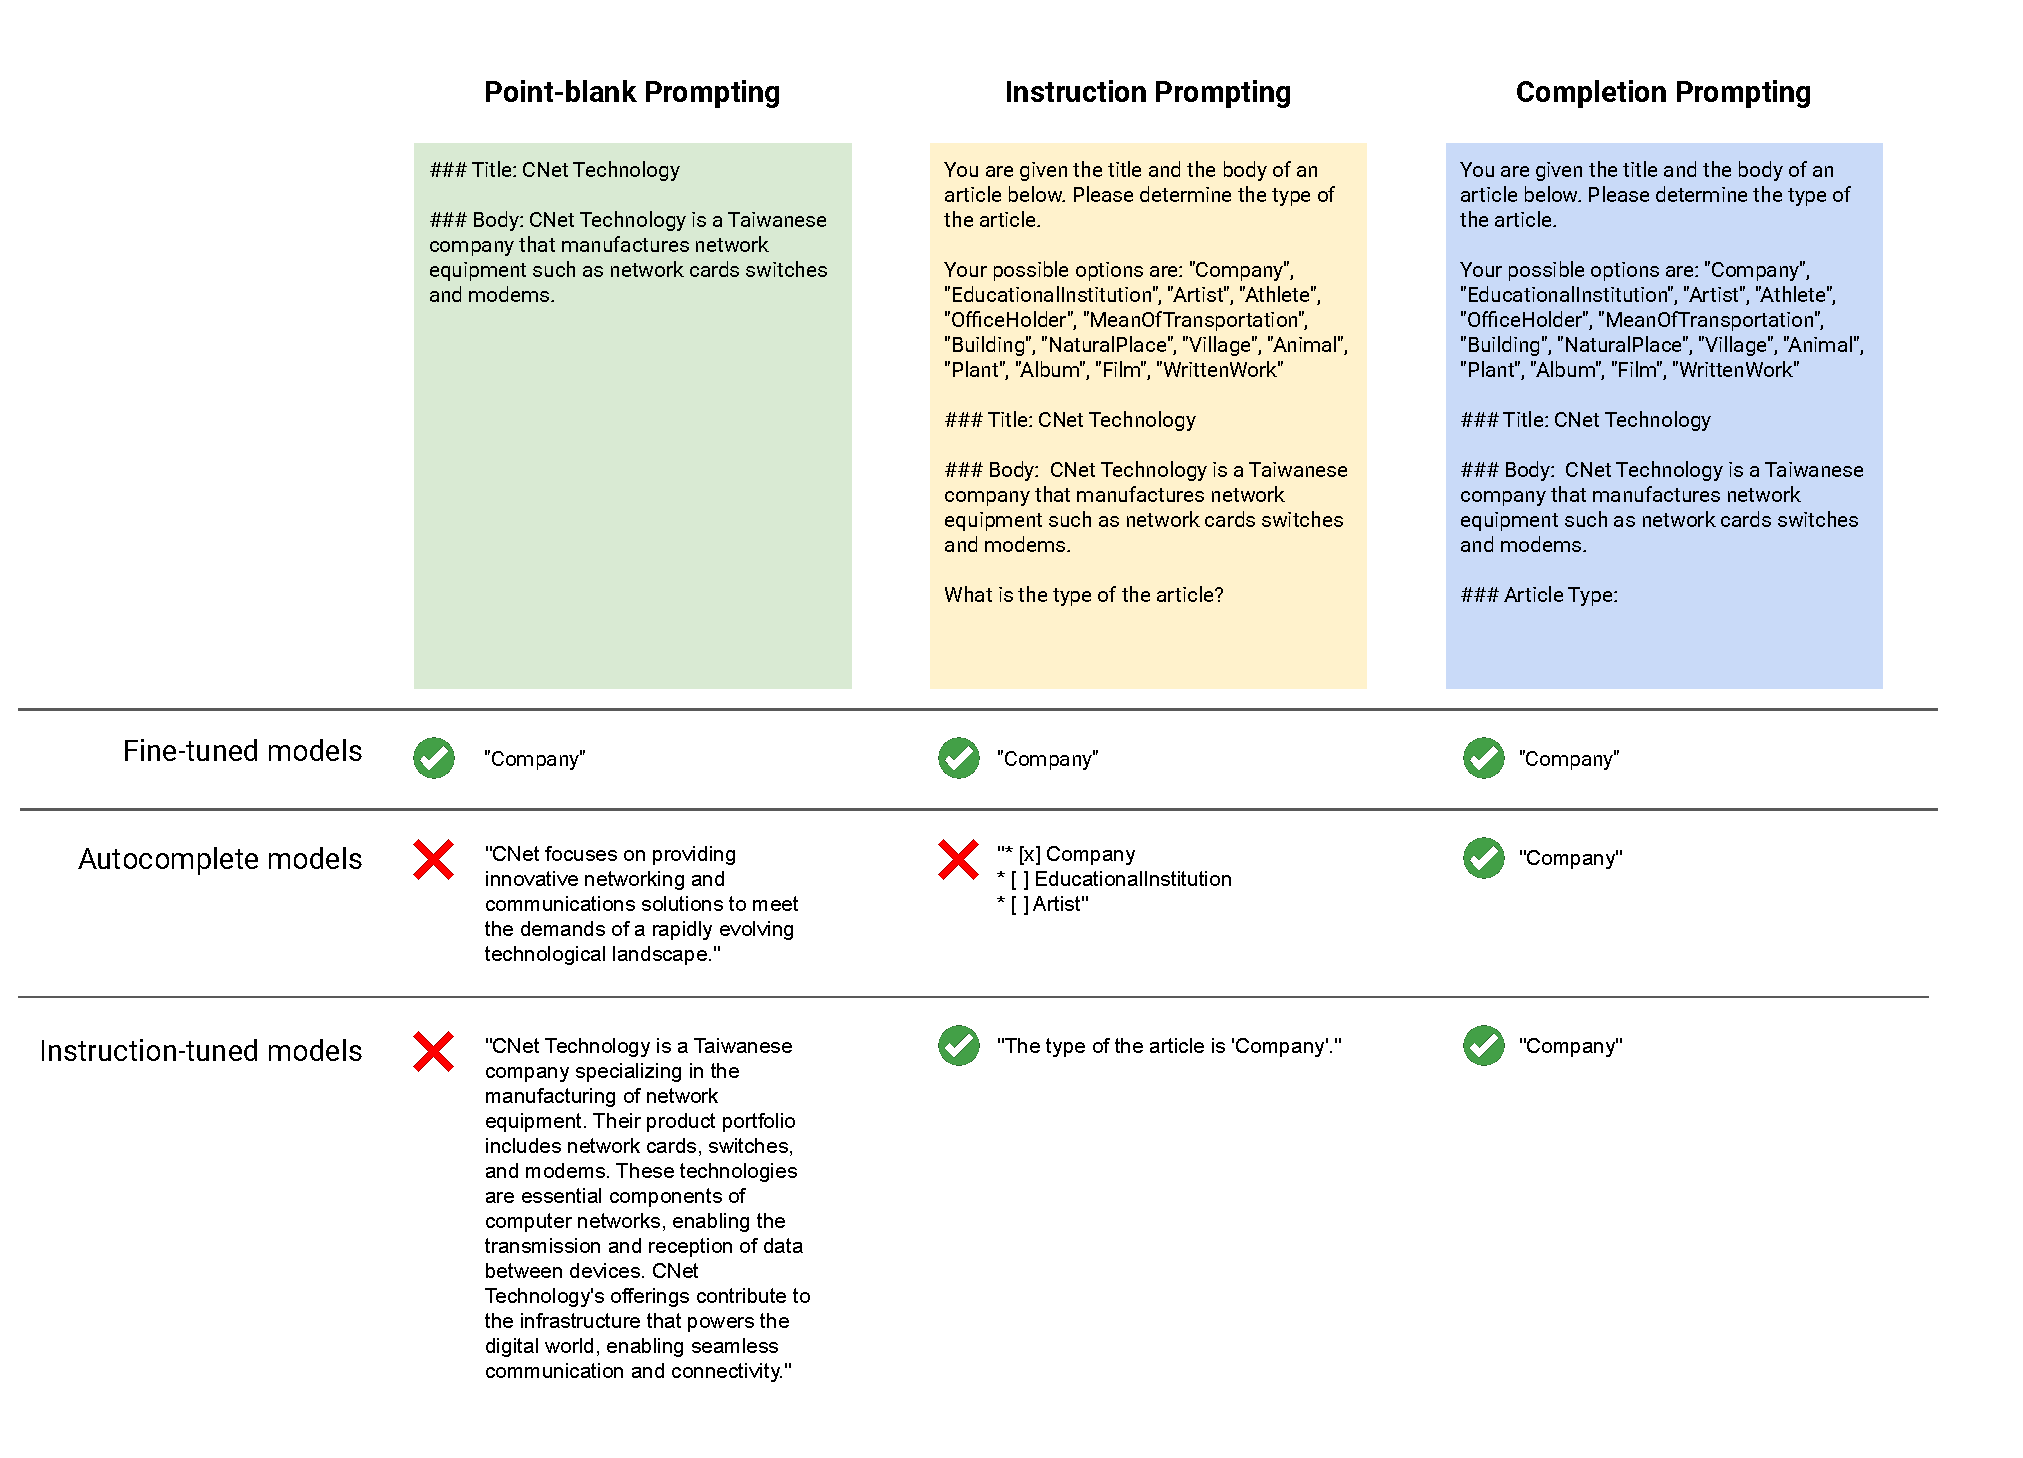
\includegraphics[width=\textwidth]{figures/prompt_design.pdf}
    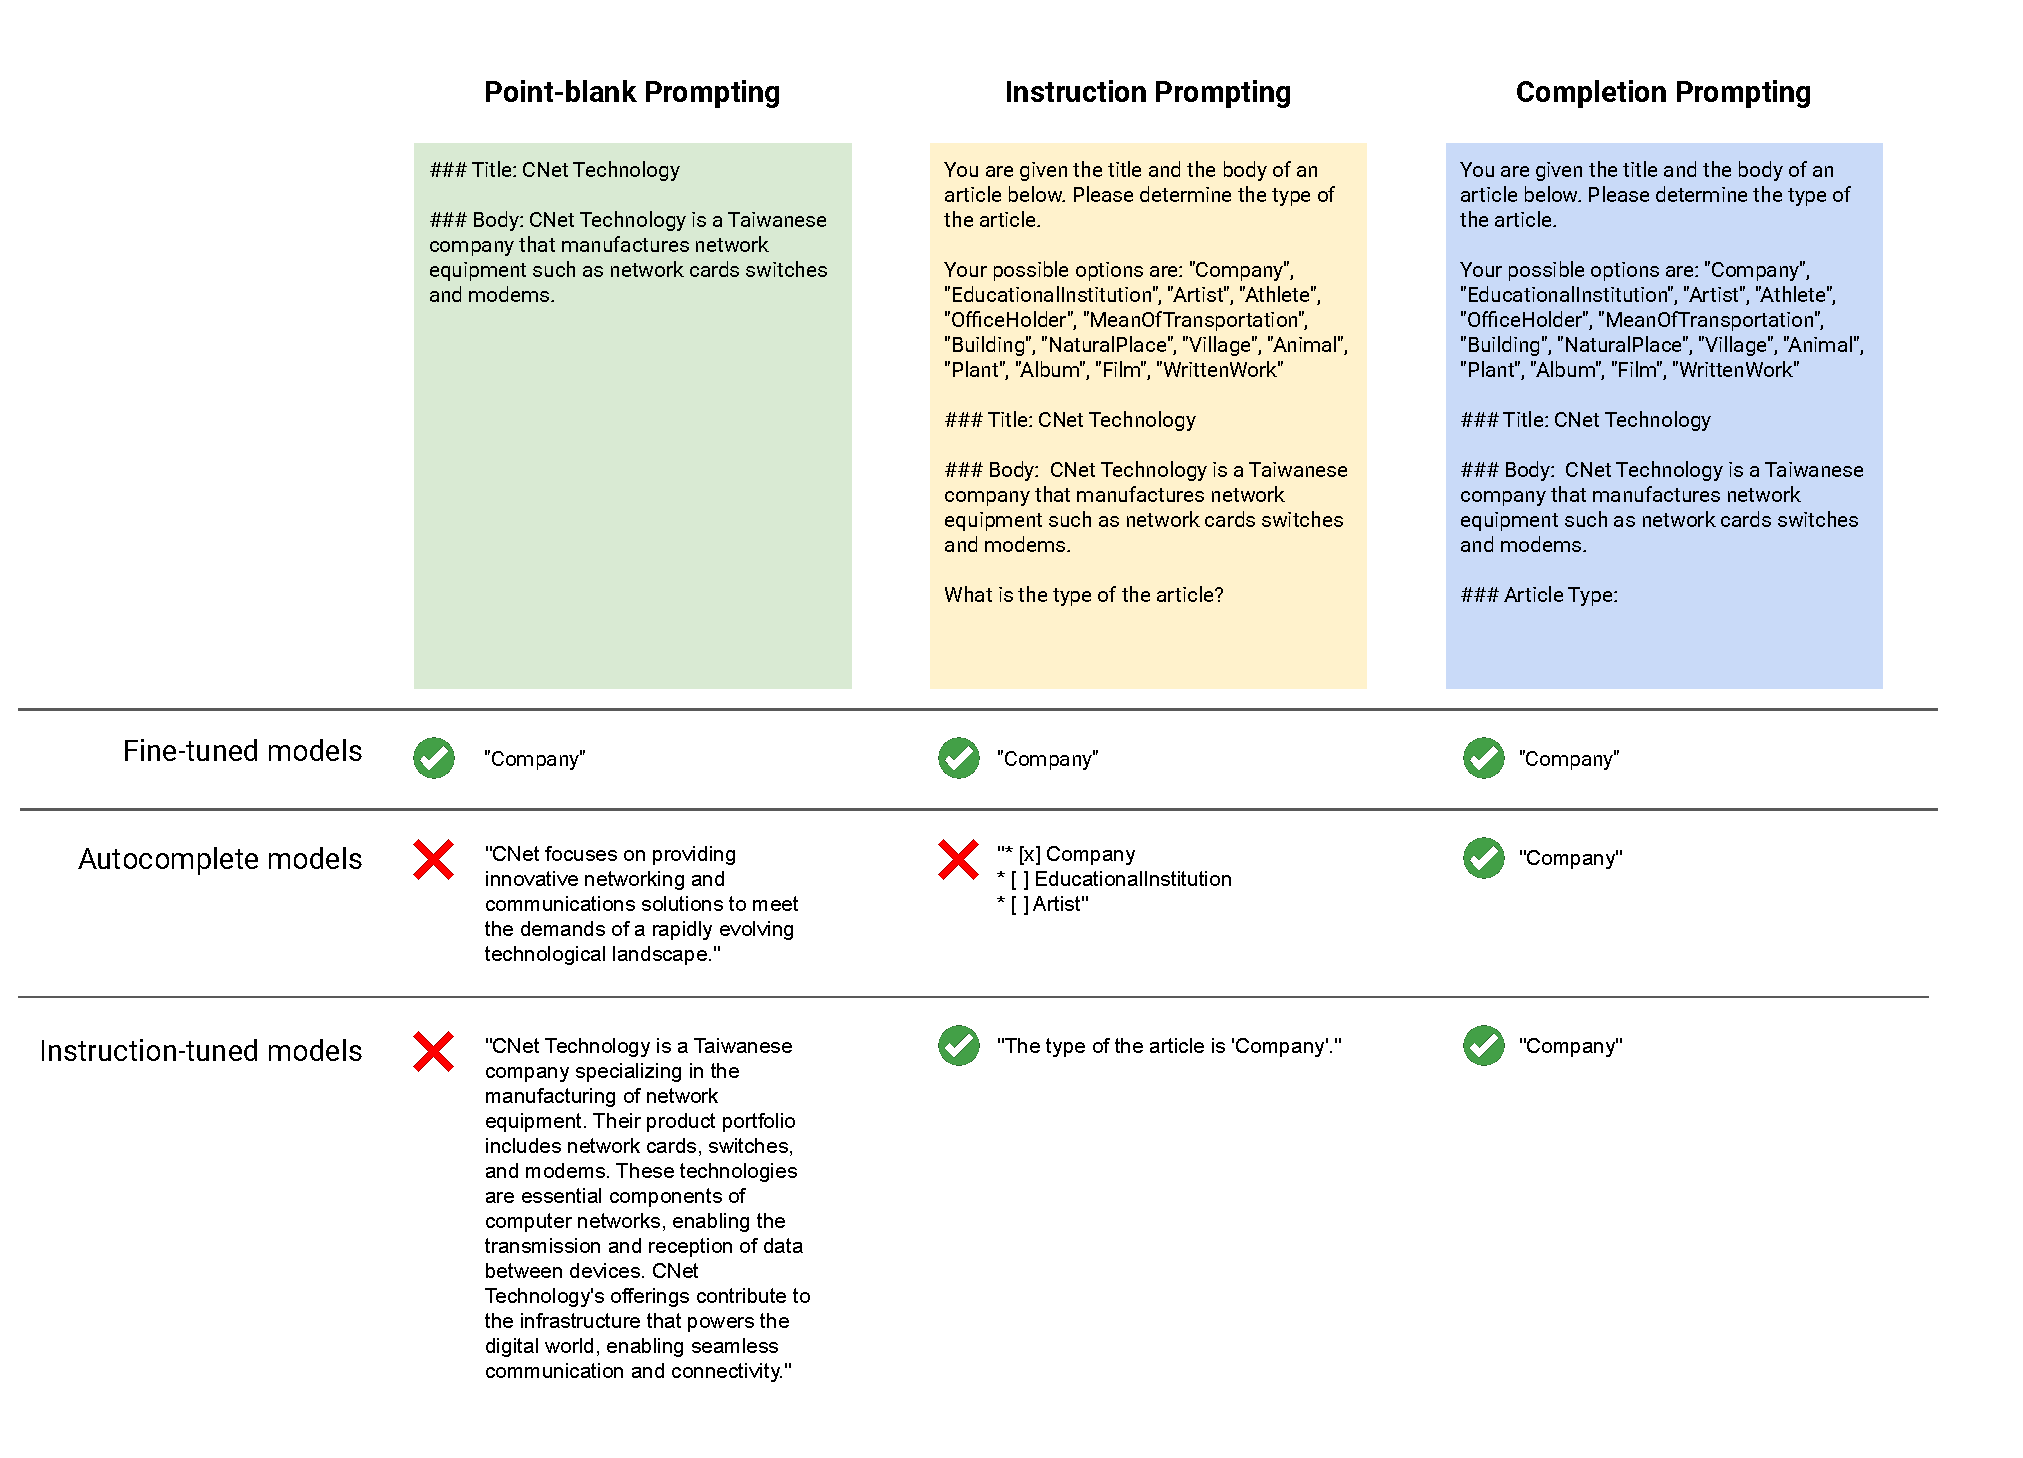
\includegraphics[width=\textwidth]{figures/prompt_design.pdf}
    \caption{Examples of different styles of prompting. To maintain using the same prompts when comparing models and to ensure the highest likelihood of success amongst all types of models (fine-tuned, auto-complete, or instruction-tuned), all of our prompts adhere to completion style.}
    \label{fig:promptdesign}
\end{figure}

Previous studies have demonstrated the potential of leveraging prompt engineering techniques, such as the use of majority voting [48], the inclusion of multiple in-context examples (n-shot)~\cite{37song2022evalsurvey}, MedPrompt~\cite{33nori2023generalistvsfinetuned}, chain-of-thought prompting~\cite{36wei2022cot}, etc., to enhance model performance on specific tasks. 

In our evaluations, we consciously choose \textbf{not} to employ additional prompt engineering or tuning strategies for any specific dataset, task, or model. Although using more in-context examples or a more selective approach in n-shot prompting might yield better results, we prioritize reproducibility and the minimization of biases that could arise from customized in-context learning. Instead, we opt to use simple zero or single-shot completion-style prompts for all tasks. Our prompts are written in the completion style, described in Figure \ref{fig:promptdesign}, to provide a fair comparison across fine-tuned, instruction-tuned, and auto-complete models. For classification tasks, the prompt includes all possible classes to inform the model's responses. For more specialized tasks, where describing the expected output format is challenging, we use a single in-context example -- the first example from the published training split -- to guide the model. 


\begin{table}[ht]

    \centering
    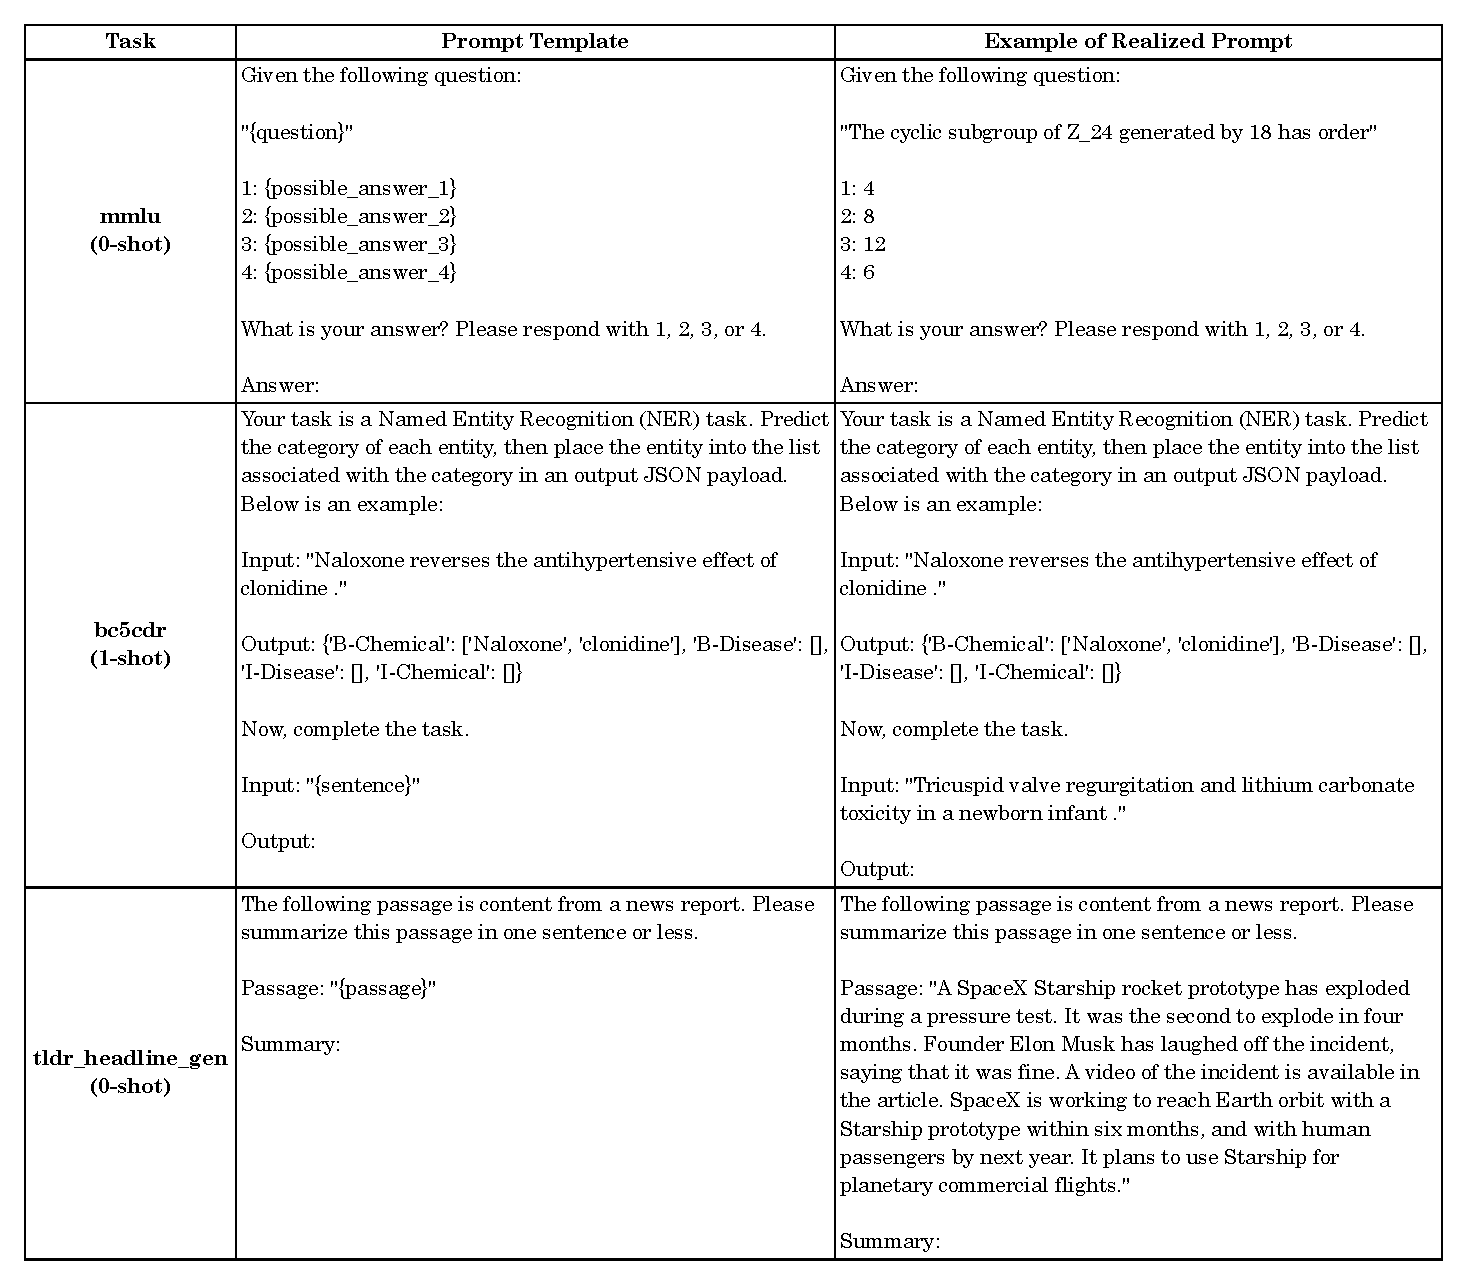
\includegraphics[width=\textwidth]{figures/prompt_template_design_examples.pdf}
    \caption{Examples of prompts that are used in this study, all written in completion style. For more specialized tasks, where describing the expected output format is challenging (e.g. \textit{bc5cdr}), we use a single in-context example — the first example from the published training split — to guide the model.}

\end{table}

Finally, we follow prescribed prompt tagging conventions for each model, as outlined in the respective model's documentation on HuggingFace, to ensure proper querying of pre-trained and instruction-tuned base models. This includes using \textbf{"<s>[INST] ... [/INST]"} for prompts intended for Mistral Instruct, and \textbf{"<bos><start\_of\_turn>user ... <end\_of\_turn><start\_of\_turn><model>"} for Gemma's instruction-tuned models.
For detailed information on the exact prompt templates applied to each task and model, please see Appendix \ref{sec:appendixprompts}.

\subsection{Base models}

All base models are listed in Table \ref{table:basemodels}. We use GPT-4 (gpt-4-0613) and GPT-3.5-Turbo (gpt-3.5-turbo-0125) as two strong LLM baselines. Our selection of these ten base models was guided by several key considerations, including their widespread adoption within the AI community, availability with permissive licenses, and availability of technical reports. We specifically choose base models with $\leq 8$ billion parameters to ensure that each model can be efficiently trained within the resource limits of a single A10G GPU. 

\begin{table*}[ht]
\centering  
\footnotesize % Smaller font size to fit the table within the page width
\begin{tabular}{llll}
\textbf{Model Name}      & \textbf{Creator} & \textbf{\# of Parameters} & \textbf{Date Released} \\
\midrule
Llama-2-7b               & Meta             & 7B                        & July 18, 2023          \\
Llama-2-7b-chat          & Meta             & 7B                        & July 18, 2023          \\
Mistral-7b-v0.1          & Mistral AI       & 7.24B                     & September 20, 2023     \\
Mistral-7b-Instruct-v0.1 & Mistral AI       & 7.24B                     & September 27, 2023     \\
Zephyr-7b                & Hugging Face     & 7.24B                     & October 26, 2023       \\
Phi-2b                   & Microsoft        & 2.78B                     & December 13, 2023      \\
Gemma-2b                 & Google           & 2.51B                     & February 21, 2024      \\
Gemma-2b-it              & Google           & 2.51B                     & February 21, 2024      \\
Gemma-7b                 & Google           & 8.54B                     & February 21, 2024      \\
Gemma-7b-it              & Google           & 8.54B                     & February 21, 2024     
\end{tabular}

\caption{Base models used in LoRA-based fine-tuning experiments. To train all models on A10G hardware, all chosen base models are ~7B parameters or smaller.}
\label{table:basemodels}
\end{table*}

\subsection{Training parameters}

Each model is trained with published train splits\footnote{\textit{customer\_support} and \textit{legal} are the only two tasks in our list without official splits. The exact splits for these datasets are published on <\href{github.com/predibase/lora-bakeoff}{github.com/predibase/lora-bakeoff}>.}. Each model is trained for $40000$ training steps with batch size 1, 4-bit quantization using bitsandbytes and a LoRA rank of $8$. We use the paged adam optimizer\cite{11dettmers2023qlora}, a learning rate of $0.002$, and a cosine learning rate scheduler with a $0.03$ warm-up fraction ($1200$ training steps). Gradients are applied over $16$ accumulation steps for an effective batch size of $16$.

These training parameters, combined with gradient checkpointing, allow each LLM to be fine-tuned on a single A10 GPU with 24 GB of memory. For tasks where training on the full sequence lengths would still produce a GPU Out-Of-Memory (OOM) error, we first truncate example inputs to a maximum sequence length set as the 95th percentile of all task inputs.

To guarantee a consistent and straightforward basis of comparison across models, no additional hyperparameter tuning is applied to any specific dataset, task, or base model.

Training recipes for each model are provided as Ludwig~\cite{62Molino2019} configurations for each of the fine-tuned LLMs and can be found at \href{https://huggingface.co/predibase}{https://huggingface.co/predibase}. Figure \ref{fig:sampleconfig} shows an example of a config.

\begin{figure}[ht]
    \centering
    \scalebox{0.5}{
    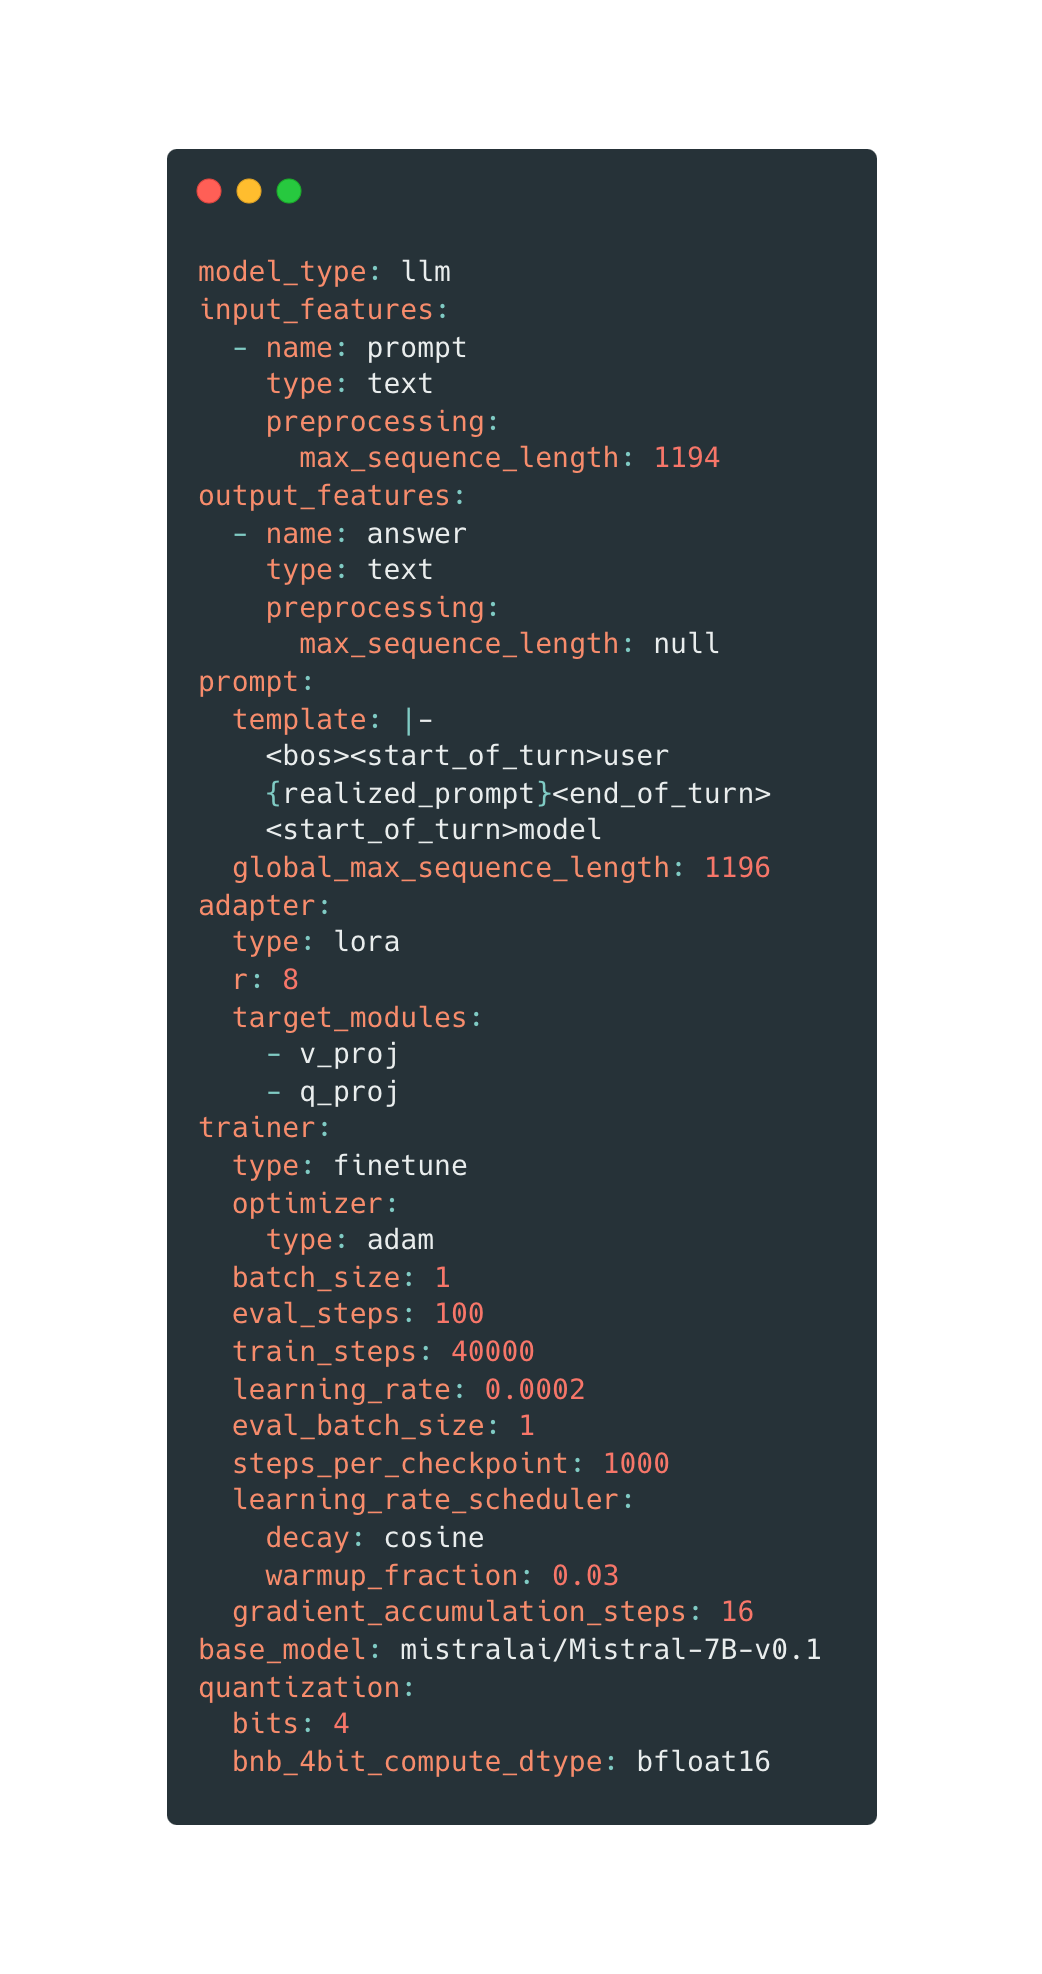
\includegraphics[width=\textwidth]{figures/ludwig_config.png}
    }
    \caption{Example LLM model training configuration for LoRA-based fine-tuning. Based on Ludwig \protect\cite{62Molino2019}.}
    \label{fig:sampleconfig}
\end{figure}

\subsection{Evaluation}

As specified in Table \ref{table:datasets}, models are evaluated on the test split if it exists and is labeled, or the validation set otherwise\footnote{MMLU has a published test set with labels, however, we use validation split to be consistent with the HELM benchmark~\cite{liang2023helm}}. We employ a tailored set of evaluation metrics to accurately assess the performance across all of the tasks. We use accuracy for classification tasks, (1 - mean absolute error) for regression tasks\footnote{Mean absolute error (MAE) is used because the range of target values are integer-like and small.}, and rouge-L\footnote{Text generation tasks are complicated to evaluate automatically~\cite{53kocmi2021nmteval}. ROUGE-L is a widely adopted proxy metric that focuses on the longest common subsequence between the generated text and the reference text, which captures the semantic similarity between the generated and reference texts rather than relying solely on exact word matches. ROUGE-L may not fully capture aspects like fluency, coherence and should be used in conjunction with other metrics and human evaluations to provide a fuller assessment of text generation quality.} for generation tasks. The WikiSQL dataset has its own \href{https://github.com/salesforce/WikiSQL/tree/master}{evaluation suite}, however due to challenges integrating the WikiSQL evaluation suite, we have adopted the ROUGE metric as a proxy for assessing query quality\footnote{Although ROUGE is not tailored for SQL queries, it offers a viable alternative for gauging the alignment between generated and target queries.}. For coding, we use HumanEval~\cite{59chen2021codex}. For GSM8K~\cite{gsm8k}, a regex-based heuristic~\cite{47eval-harness} is used to extract the mathematical answer to be consistent with the Open LLM Leaderboard~\cite{34open-llm-leaderboard}. All metrics are on a 0 to 1 scale, where 0 is the worst possible score, and 1 the best possible score.

Non-fine-tuned models often generate more varied outputs, including unintended artifacts such as additional words or explanations not specified in the prompt. For classification tasks, sometimes these models will generate the actual class string like "Yes/No", "positive/negative" or "True/False" spelled out, instead of the true "1/0" label in the dataset even when instructed. To minimize metric deductions due to response parsing strictness, we first use a regex-based extraction step to map the model’s response to the ground truth vocabulary. If there are multiple matches in the generated text, the first valid match is used. The code for regex-based pre-metric response extractions are available at \href{https://www.github.com/predibase/lora-bakeoff}{github.com/predibase/lora-bakeoff}.

Financial constraints associated with LLM APIs are not trivial. For example, using GPT-4 to assess the complete WikiSQL test set of 15,878 examples would cost approximately \$400, considering the average input (805) and output (16) token counts per example. Such costs can be prohibitive, especially for organizations or researchers operating on limited budgets.

To manage costs while maintaining rigor, we restrict evaluations to the \textbf{first} 1000 examples for datasets with evaluation splits larger than 1000 examples. We acknowledge that this method may introduce selection bias and affect the generalizability of our findings. We recommend that future research considers more expansive evaluations as resources permit.
